Dieses Kapitel beschreibt die Planung des Projekts, welche zu Projektbeginn definiert wurde.
Es wurde ein Projektplan erarbeitet und Meilensteine zur Fortschrittskontrolle erfasst.

\subsection{Projektplan}

Der Projektplan wurde zu Beginn der Projektarbeit definiert und wie in Abbildung 2.1 dargestellt festgehalten.
Folgendes Kapitel beschreibt den damit definierten Ablauf.

\begin{figure}[h]
    \centering
    \begin{minipage}[b]{\textwidth}
        \fbox{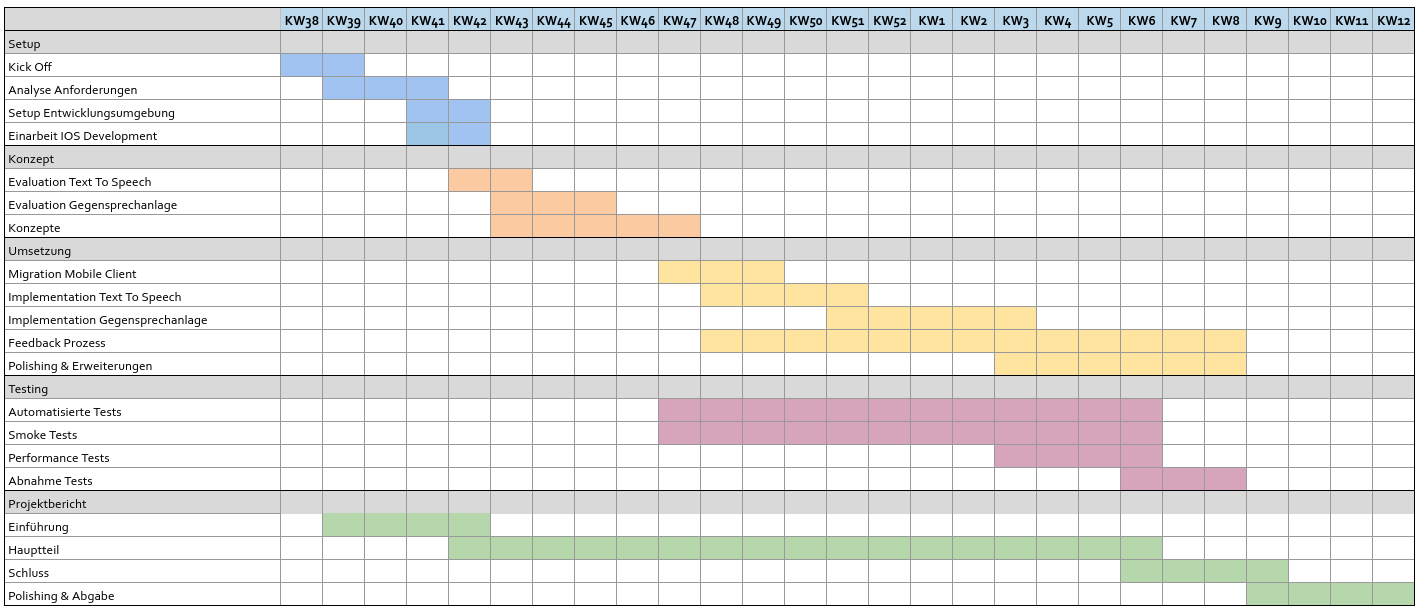
\includegraphics[width=\textwidth]{graphics/projektplan}}
        \caption{Projektplan}
    \end{minipage}\label{fig:projektplan}
\end{figure}

Das Projekt beginnt mit einer Setup-Phase.
Anforderungen und Umfang des Projektes werden zusammen mit dem Auftraggeber erarbeitet und dokumentiert.
Es wird ein Projektplan erstellt und die grobe Struktur des Projektberichts definiert.
Infrastruktur und Codebasis des Vorgängerprojektes wird übernommen und wo nötig für dieses Projekt angepasst.
Für die Entwicklung einer nativen iOS App muss eine Entwicklungsumgebung inklusive Hardware und Testgeräten aufgesetzt werden.
Während dieser Zeit findet bereits eine Einarbeitung in native iOS Entwicklung statt.
So können erste Erfahrungen gesammelt werden und die Vollständigkeit der Entwicklungsumgebung validiert werden.
Nach der Setup-Phase beginnt die Konzept-Phase.
Dies beinhaltet Evaluation von Technologien sowie Definition von Grundprozessen und Datenstrukturen.
Die erstellten Konzepte werden mit einfachen gehaltenen Proof Of Concepts validiert.
Alle erarbeiteten Konzepte werden dokumentiert.
Es wird beschrieben, wie die bestehende Systemarchitektur erweitert wird, um die neuen Funktionen integrieren.
Dabei müssen insbesondere Skalierbarkeit, Erweiterbarkeit und Integrierbarkeit des Systems bewahrt werden.
Die Umsetzung des Systems findet schliesslich in der dritten Phase.
Die erarbeiteten Konzepte werden umgesetzt und in das Praxisrufsystem integriert.
Bei der Umsetzung wird als Erstes der bestehende Mobile Client als native iOS Applikation neu entwickelt.
Darauf werden Sprachsynthese und letztlich Gegensprechanlage implementiert.
Die erarbeiteten Konzepte werden dabei laufend verfeinert und wo nötig angepasst.
Während der Umsetzung wird der aktuelle Stand regelmässig mit dem Kunden besprochen.
Der Kunde kann so frühzeitig Rückmeldung geben.
Gewünschte Anpassungen und Erweiterungen können Frühzeitig eingeplant werden.
Parallel zur Umsetzung läuft eine Testing-Phase.
Diese beinhaltet das Schreiben von automatisierten Tests und regelmässigen manuellen Tests des aktuellen Stands.
Zum Ende der Umsetzungsphase wird schliesslich ein Abnahmetest mit dem Kunden durchgeführt.
Die vierte Phase bildet den Abschluss des Projekts.
Es werden keine Änderungen mehr an der Applikation vorgenommen.
Der Projektbericht wird fertiggestellt und das Projekt wird für die Abgabe vorbereitet.

